\chapter{High Availability Deployments}
\label{sec:high-availability}


\cxoneflow can be deployed in a high-availability configuration using multiple instances of
the \cxoneflow container.  The \cxoneflow instances need to have a shared MQ cluster that
can communicate with the AMQP protocol.  The MQ instance is where long-running state data
is persisted by each instance.  Figure \ref{fig:ha-diagram} shows a deployment diagram for
a typical high-availability configuration.


\begin{figure}[h]
    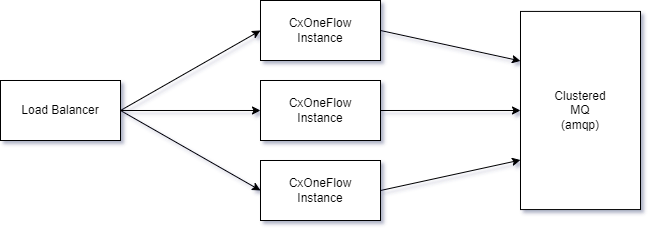
\includegraphics[width=\textwidth]{graphics/cxoneflow-diagrams-HA.png}
    \caption{High Availability Deployment Diagram}
    \label{fig:ha-diagram}
\end{figure}


\noindent\\The user account connected to the MQ must have the ability to configure the
exchange and queue schema.  Configuration generally does not require administrative privileges.

\noindent\\The \texttt{/ping} endpoint on the \cxoneflow container can be used
for health-check by the load balancer.


